\documentclass[aspectratio=169]{beamer}
\usepackage{dbt}

%%%% Standard packages
\usepackage{graphicx}
\usepackage{epstopdf}
\usepackage{multirow}
\usepackage{cancel}
\usepackage{bm} % bold math
\usepackage[squaren,thickqspace]{SIunits}
% \usepackage{animate}
% Packages for typesetting algorithms and good looking pseudocode 
\usepackage{algorithm}
\resetcounteronoverlays{algorithm}
\usepackage[noend]{algpseudocode}
% Handling tables
\usepackage{wrapfig}
\usepackage{macros}

%%%% TIKZ
\usepackage{tikz}
\usepackage{caption}
\usetikzlibrary{decorations.pathreplacing,shapes,arrows,positioning}
\tikzset{
	vertex/.style = {
		circle,
		fill            = black,
		outer sep = 2pt,
		inner sep = 1pt,
	}
}
\usetikzlibrary{spy}
\usetikzlibrary{matrix}
\usetikzlibrary{overlay-beamer-styles}

% Handling units
\usepackage[thickqspace]{SIunits}
\addunit{\pixel}{pixel}
\addunit{\pixels}{pixels}
\addunit{\voxel}{voxel}
\addunit{\decibel}{dB}
\addunit{\byte}{B}
\addunit{\hounsfield}{HU}

\setbeamercolor{emph}{fg=hilight}
\renewcommand<>{\emph}[1]{%
	{\usebeamercolor[fg]{emph}\only#2{\itshape}#1}%
}

\setbeamercolor{alert}{fg=vhilight}
\renewcommand<>{\alert}[1]{%
	{\usebeamercolor[fg]{alert}\only#2{\itshape}#1}%
}

\setbeamercolor{structure}{fg=title}
\renewcommand<>{\alert}[1]{%
	{\usebeamercolor[fg]{alert}\only#2{\itshape}#1}%
}

\setbeamercolor{section in head/foot}{fg=title}
\setbeamertemplate{footline}
{
	\leavevmode%
	\hbox{%
		\begin{beamercolorbox}[wd=.333333\paperwidth,ht=2.25ex,dp=1ex,center]{section in head/foot}%
			\usebeamerfont{author in head/foot}\insertshortauthor
		\end{beamercolorbox}%
		\begin{beamercolorbox}[wd=.333333\paperwidth,ht=2.25ex,dp=1ex,center]{section in head/foot}%
			\usebeamerfont{title in head/foot}\insertshorttitle
		\end{beamercolorbox}%
		\begin{beamercolorbox}[wd=.333333\paperwidth,ht=2.25ex,dp=1ex,right]{section in head/foot}%
			\usebeamerfont{date in head/foot}\insertshortdate{}\hspace*{2em}
			\insertframenumber{} / \inserttotalframenumber\hspace*{2ex} 
		\end{beamercolorbox}}%
		\vskip0pt%
}
\makeatother

% Semi-visible itemize
\setbeamercovered{invisible}
\setbeamercovered{%
	again covered={\opaqueness<1->{40}}}

% backup slides
\newcommand{\backupbegin}{
	\newcounter{framenumberappendix}
	\setcounter{framenumberappendix}{\value{framenumber}}
}
\newcommand{\backupend}{
	\addtocounter{framenumberappendix}{-\value{framenumber}}
	\addtocounter{framenumber}{\value{framenumberappendix}} 
}

% Listing
\usepackage{listings}

% Declare image layers
% By default all math in TikZ nodes are set in inline mode. Change this to
% displaystyle so that we don't get small fractions.
\everymath{\displaystyle}

%%%% Macros 
% Sets
\newcommand\datamanifold{\mathbb{M}}
\newcommand\trainingdata{\mathcal{M}}
% Spaces
\newcommand{\ParamSpace}{\ensuremath{Z}}
\newcommand{\ProdSpace}{\ensuremath{U}}
\newcommand{\FeatureSpace}{\ensuremath{\mathbb{F}}}
% Operators
\newcommand{\approxInv}[1]{#1^{\dagger}}
\newcommand{\learnedInv}[1]{#1^{\dagger}}
\DeclareMathOperator{\IdentityOp}{\ensuremath{\text{Id}}}
\DeclareMathOperator{\OpA}{\ensuremath{\mathcal{A}}}
\DeclareMathOperator{\OpB}{\ensuremath{\mathcal{B}}}
\DeclareMathOperator{\OpC}{\ensuremath{\mathcal{C}}}
\DeclareMathOperator{\OpF}{\ensuremath{\mathcal{F}}}
\DeclareMathOperator{\OpG}{\ensuremath{\mathcal{G}}}
\DeclareMathOperator{\OpK}{\ensuremath{\mathcal{K}}}
\DeclareMathOperator{\ForwardOpPseudoInv}{\ensuremath{\approxInv{\ForwardOp}}}
\DeclareMathOperator{\ForwardOpInvLearned}{\ensuremath{\learnedInv{\ForwardOp}_{\param}}}
\DeclareMathOperator{\RadonTransform}{\ensuremath{\mathcal{P}}}
\DeclareMathOperator{\LogLikelihood}{\ensuremath{\mathcal{L}}}
\DeclareMathOperator{\AffineOp}{\ensuremath{\mathcal{W}}}
\DeclareMathOperator{\NonLinOp}{\ensuremath{\OpA}}
\DeclareMathOperator{\errorfunc}{E}
\DeclareMathOperator{\RegOp}{\mathcal{S}}
\DeclareMathOperator{\loss}{L}
\DeclareMathOperator{\objective}{\mathcal{E}}
\DeclareMathOperator{\distance}{d}
\DeclareMathOperator{\grad}{\nabla\!}
\DeclareMathOperator{\ProxOp}{\ensuremath{prox}}
\DeclareMathOperator{\esssup}{\ensuremath{ess\,sup}}
\DeclareMathOperator{\FeatureExt}{\ensuremath{\mathcal{R}}}
% Probabilistic concepts
\newcommand{\stochastic}[1]{\mathsf{#1}}
\newcommand{\stsignal}{\stochastic{\signal}}
\newcommand{\stdata}{\stochastic{\data}}
\DeclareMathOperator{\ProbdistFunctional}{\stochastic{F}}
\DeclareMathOperator{\Expect}{\mathbb{E}}
\DeclareMathOperator{\Variance}{Var}
\newcommand{\ProbabilityDistribution}{\stochastic{P}}
\newcommand{\ProbabilityMeasure}{\mu}
% Elements in spaces
\newcommand{\signal}{\ensuremath{f}}
\newcommand{\signalother}{\ensuremath{h}}
\newcommand{\signaltrue}{\signal_{\text{true}}}
\newcommand{\mollifier}{\ensuremath{e}}
\newcommand{\noise}{\delta\data}
\newcommand{\signallearned}[1]{\ForwardOpInvLearned(#1)}
\newcommand{\memory}{s}
\newcommand{\param}{\ensuremath{\theta}}
\newcommand{\weight}{\ensuremath{w}}
\newcommand{\vweight}{\ensuremath{\boldsymbol{\weight}}}
\newcommand{\bias}{\ensuremath{b}}
\newcommand{\primal}{\ensuremath{f}}
\newcommand{\dual}{\ensuremath{h}}
\newcommand{\beameritemnestingprefix}{}
%\newcommand{\leadsto}{\rightsquigarrow}

\title[ODL]{{\Huge ODL}\\ {\large A Python framework for rapid prototyping in inverse~problems}}
\author[Jonas Adler (\texttt{jonasadl@kth.se})]{Jonas Adler\inst{1, 2} \and Holger Kohr\inst{3} \and Ozan \"{O}ktem\inst{1}}
\institute{
\inst{1} Department of Mathematics \\ KTH - Royal Institute of Technology, Stockholm
\and %
\inst{2} Research and Physics \\ Elekta, Stockholm
\and %
\inst{3} Thermo Fisher Scientific, Eindhoven}
\date{}
\titlegraphic{%
  
\includegraphics[height=40pt]{images/KTH_Logotype}\hspace*{1.0cm}~%
  
\includegraphics[height=40pt]{images/Elekta-vertical}\hspace{1.0cm}%
  
\includegraphics[height=25pt]{images/Thermo_Fisher_Scientific_logo}\hspace{1.0cm}%
  
\includegraphics[height=40pt]{images/SSF_Logotype}
}
\begin{document}
  
\begin{frame}[plain]
  \titlepage
\end{frame}

\begin{frame}
\frametitle{Why a new software framework?}

\begin{itemize}
  \item<+> \structure{Multiple modalities:} CT, CBCT, PET, SPECT, spectral CT, phase contrast CT, electron tomography, MRI, HADAF-STEM \ldots
  \item<+> \structure{Collaborative research:} Need to share implementations of common concepts
  \item<+> \structure{Reproducible research:} Not enough to share theory and pseudocode, also need to share data and concrete implementations \\
  $\leadsto$ Software components need to be usable by others.
  \item<+> \structure{Flexibility:} Mathematical structures/notions \emph{re-usable across modalities} \\
 $\leadsto$ Make it easy to ``play around'' with new ideas and combine concepts.
\end{itemize}
\visible<5->{
\structure{Conclusion:}
Need a \emph{common software framework} to exchange implementations of concepts and methods.
}
\end{frame}

\begin{frame}
\frametitle{Why a new software framework?}

\structure{Requirements on a software framework:}

\begin{itemize}
 \item<+> Allow formulation and solution of inverse problems in a \emph{common language}.
 \item<+> Make implementations \emph{re-usable} and \emph{extendable}.
 \item<+> Enable \emph{fast prototyping} on \emph{clinically relevant data}.
 \item<+> Leverage the power of \emph{existing libraries}.
\end{itemize}

\visible<5->{\structure{Initial situation:} No existing framework fit our purpose.}

\end{frame}


\begin{frame}{Operator Discretization Library}

  \structure{Main components:}
  \begin{overprint}
    \onslide<1-3>
    \begin{itemize}
      \item<+> \structure{Functional analysis module}\\
      Handling of \emph{vector spaces}, \emph{operators}, \emph{discretizations} -- generally with a \emph{continuous} point of view

      \item<+> \structure{Optimization methods module}\\
      \emph{General-purpose} optimization methods suitable for solving inverse problems.

      \item<+> \structure{Tomography module}\\
      Acquisition \emph{geometries} and \emph{forward operators} for tomographic applications.
    \end{itemize}
    
    \onslide<4-5>
    \begin{itemize}
      \item<+> \structure{Library of atomic mathematical components}
      {\small
      	\\-- Deformation operators
    	\\-- Function transforms: wavelet, Fourier, shearlet, \dots
	    \\-- Differential operators: partial derivative, gradient,  Laplacian, \dots
	    \\-- Discretization-related: (re-)sampling, interpolation, domain extension, \dots
      }
      \item<+> \structure{Utility functions}
      {\small 
      	\\-- Visualization: Slice viewer, real time plotting, \dots
      	\\-- Phantoms: Shepp-Logan, FORBILD, Defrise, \dots
      	\\-- Data I/O: MRC2014, Mayo Clinic, \dots
      }
    \end{itemize}
    
    \onslide<6->
    \begin{itemize}
      \item \structure{User-contributed modules} \\
	      ``Fast track'' for experimental or slightly exotic code
	    {\small 
		    \\-- Figures of Merit (FOMs) for image quality assessment
			\\-- Handlers for specific data formats or geometries
			\\-- Functionality to download and import public datasets
			\\-- Wrappers for Deep Learning frameworks: Tensorflow, Theano, Pytorch, \dots
		}
    \end{itemize}
  \end{overprint}%
\end{frame}


\begin{frame}{Design principle: modularity}
  Consider a TV minimization problem
  %
  \begin{equation*}
    \min_{f \in \SPCX} \left[\NORM{\OPT(f) - g}_\DataSpace^2 + \lambda \TV(f)  \right]
  \end{equation*}
  \vspace*{-0.5ex}%
  \structure{Components:} \\[1ex]
  \begin{minipage}{0.42\textwidth}
    \begin{itemize}
      \item<+-> Reconstruction space $\SPCX$
      \item<+-> Data space $\DataSpace$
      \item<+-> Forward operator $\OPT \colon \SPCX \to \DataSpace$
      \item<+-> Data $g \in \DataSpace$
    \end{itemize}
  \end{minipage}
  %
  \begin{minipage}{0.52\textwidth}
    \begin{itemize}
      \item<+-> Data discrepancy functional $\NORM{\,\cdot - g}_\DataSpace^2$
      \item<+-> Regularization parameter $\lambda > 0$
      \item<+-> Regularization functional $\TV(\cdot)$
    \end{itemize}
    \vspace*{14pt}
  \end{minipage}
  %
  \vspace*{2ex}
  %
  \begin{itemize}
    \item<+>[$\leadsto$] (almost) freely exchangeable ``modules'' in the mathematical formulation
    \item<+>[$\leadsto$] ODL maps them to software objects as closely as possible
    \item<+>[$\leadsto$] Mathematics as strong guideline for software design
    \item<+>[$\leadsto$] Makes the software ``feel'' natural
  \end{itemize}

\end{frame}


\begin{frame}{Design principle: abstraction}

  \uncover<+->{%
  \structure{Landweber's method}: Determine $f$ from given data $g = \OPT(f)$ and initial guess $f_0$ by
  %
  \begin{equation*}
  f_{k+1} = f_k + \omega [\partial\!\OPT(f_k)]^*\big(g - \OPT(f_k) \big),\quad k = 0, 1, \ldots, K-1
  \end{equation*}
  }%
  %
  \vspace*{-1ex}%
  \uncover<+->{%
  \lstinputlisting[%
    language=Python,basicstyle=\footnotesize\ttfamily,%
    keywordstyle=\bfseries\color{green!20!blue},%
    commentstyle=\itshape\color{green!50!white},%
    stringstyle=\color{orange}%
  ]%
  {code/landweber.py}
  }
  %
  \begin{itemize}
  \item<+>
    Completely generic (expects operator, data, plus some parameters)
  \item<+>
    Uses abstract properties of operators in the iteration:
    {\small
	    \\$\leadsto$ \texttt{T(f)} $\longleftrightarrow$ $\OPT(f)$ (operator evaluation)
	    \\$\leadsto$ \texttt{T.derivative(f)} $\longleftrightarrow$ $\partial\!\OPT(f)$ (derivative \emph{operator} at $f$)
	    \\$\leadsto$ \texttt{T.derivative(f).adjoint} $\longleftrightarrow$ $[\partial\!\OPT(f)]^*$ (adjoint of the derivative at $f$)
	}
  \end{itemize}
  \vspace*{20pt}

\end{frame}


\begin{frame}{Design principle: abstraction}

  \structure{Landweber's method}: Determine $f$ from given data $g = \OPT(f)$ and initial guess $f_0$ by
  %
  \begin{equation*}
  f_{k+1} = f_k + \omega [\partial\!\OPT(f_k)]^*\big(g - \OPT(f_k) \big),\quad k = 0, 1, \ldots, K-1
  \end{equation*}
  %
  \vspace*{-1ex}%
  \lstinputlisting[%
    language=Python,basicstyle=\footnotesize\ttfamily,%
    keywordstyle=\bfseries\color{green!20!blue},%
    commentstyle=\itshape\color{green!50!white},%
    stringstyle=\color{orange}%
  ]%
  {code/landweber.py}
  %
  \begin{itemize}
    \item<+>
      \texttt{T} is an \texttt{Operator} that implements a \emph{generic, abstract} interface: \\
      \texttt{domain}, \texttt{range}, \texttt{derivative}, \texttt{adjoint}, operator \emph{evaluation}
    \item<+>
      Lots of tools to build complex operators from simple ones: \\
      operator arithmetic \texttt{T + S}, composition \texttt{T * S}, product space operators etc.
    \item<+>
      There are \emph{many} readily implement operators in ODL, all implementing the above interface
  \end{itemize}

\end{frame}


\begin{frame}{Design principle: compartmentalization}

  \begin{itemize}
    \item<+> Separates the ``what'' (abstract interface) of an object class from the ``how'' (concrete implementation) \\
    \structure{Example:} Fourier transform using \texttt{NumPy} FFT vs. \texttt{pyFFTW} vs. \texttt{cuFFT}
    \item<+> Allows building generic APIs with the possibility for a new implementation in the future (\emph{extensibility}) \\
    \structure{Example:} \texttt{L1Norm} as a concrete realization of the abstract \texttt{Functional}
    \item<+> Makes functions and classes individually testable
    \item<+> Documentation is bundled with the object and immediately visible to the user
    \item<+> Code becomes more maintainable, low risk for ``god objects'' or scope glide
  \end{itemize}

\end{frame}


%\begin{frame}{Design compromises}
%
%  \begin{itemize}
%    \item<+->
%      Distinguish types only if they have \emph{computable} differences. \\[1ex]
%      \structure{Example:} There is only one \texttt{FunctionSpace} representing $\mathcal{F}(\Omega, \FIELD) = \SET{f \colon \Omega \to \FIELD}$. \\
%      \structure{Reason:} No way to do ``interesting'' things without symbolic calculus.
%    \item<+->
%      Include only features that \emph{add value} in a specific task. \\[1ex]
%      \structure{Example:} Currently, only nearest neighbor and linear interpolation implemented. \\
%      \structure{Reason:} Higher-order schemes are seldom used in imaging, no need so far.
%    \item<+->
%      Enforce mathematical rigor only to help the users. \emph{Don't stand in their way}. \\[1ex]
%      \structure{Example:} For operator composition \texttt{T * S}, check if \texttt{S.range == T.domain}. Conversely, no convexity check of \texttt{Functional}s in optimization methods.\\
%      \structure{Reason:} Wrong domains/ranges are a major error source, checking helps users. Conversely, a convex method may work well even on a non-convex problem.
%  \end{itemize}
%
%\end{frame}

\begin{frame}{Further design considerations}

  \begin{itemize}
    \item<+>
      ODL is a \emph{prototyping} framework, not a black-box solution
      {\small
      	\\$\leadsto$ Give users freedom to experiment and tinker, do ``unorthodox'' things
        \\$\leadsto$ Very little ``intelligence'' that guesses what a user wants
        \\$\leadsto$ Instead: make things ``just work'' that a typical user would expect to work
      }

    \item<+>
      It should be \emph{fun} to explore the ``What if?'' scenarios in existing examples
    \item<+>
      Make use of external highly optimized code for heavy tasks if adequate
    \item<+>
      Don't sacrifice performance! 
      {\small
      	\\$\leadsto$ Use libraries in the most efficient way possible (avoid copies, operate in-place, work with low-dimensional arrays, vectorization, broadcasting, \dots)
	    \\$\leadsto$ Compute on the GPU whenever possible (new fast back-end coming soon)
	  }
  \end{itemize}

\end{frame}


\begin{frame}{Example: Tomography}

  \structure{Inverse Problem:} Determine attenuation coefficient $\mu \colon \Omega \to \RR$ from its ray transform $\RadonTransform \colon L^2(\Omega) \to \DataSpace$ defined as
  %
  \begin{equation*}
  	\RadonTransform(\mu)(\ell) \DEFEQ \int_\ell \mu(x) \D x
  \end{equation*}
  %
  for all lines $\ell$. \\[2ex]

  \pause
  \structure{Given:} Noisy data
  %
  \begin{equation*}
  	g(\ell) \approx \RadonTransform(\mu)(\ell)
  \end{equation*}
  % Below not necessary information in the slides, also removed indices that only confuse
  %for lines $\ell_{p,k}$ defined by directional vectors $\theta_p \in S^1$ and shifts $v_{p,k} \perp \theta_p$ (2D parallel beam geometry) \\[2ex]

  \pause
  \structure{Regularization:} Conjugate gradient (CGLS) with early termination

\end{frame}


\begin{frame}{Example: Tomography}

  \structure{Implementation steps:}

  \begin{itemize}
    \item<+> Set up uniformly \emph{discretized} image space $L^2(\domain)$ with a rectangular domain $\domain$ and $n_x \times n_y$ pixels
    \item<+> Create parallel beam geometry with $P$ angles and $K$ detector pixels
    \item<+> Define ray transform $\RadonTransform \colon L^2(\domain) \to \DataSpace$ (the space $\DataSpace$ is inferred from the geometry)
    \item<+> Solve inverse problem using CGLS
    \item<+> Display the results
  \end{itemize}

\end{frame}

\begin{frame}{Example: Tomography}
  \lstinputlisting[%
    language=Python,basicstyle=\footnotesize\ttfamily,%
    keywordstyle=\bfseries\color{green!20!blue},%
    commentstyle=\itshape\color{green!50!white},%
    stringstyle=\color{orange},%
    basicstyle=\scriptsize,%
    deletendkeywords={range}%
  ]%
  {code/tomography.py}
  %

\end{frame}


\begin{frame}{Example: Tomography}
	
	\begin{minipage}{0.31\textwidth}
		\centering
		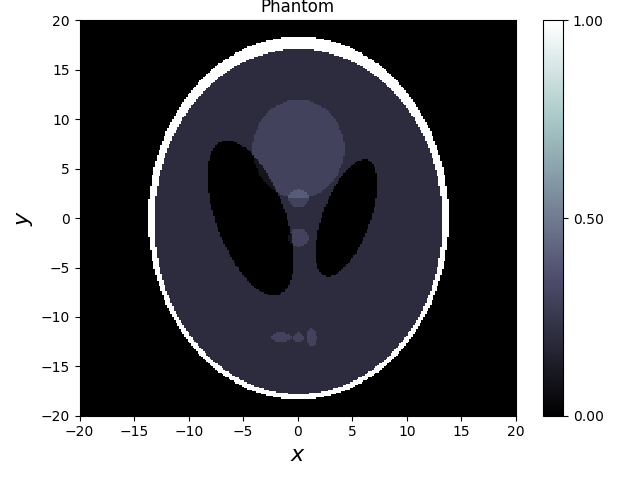
\includegraphics[width=\linewidth]{images/phantom}
	\end{minipage}
	%
	\hspace*{0.01\linewidth}
	%
	\begin{minipage}{0.31\textwidth}
		\centering
		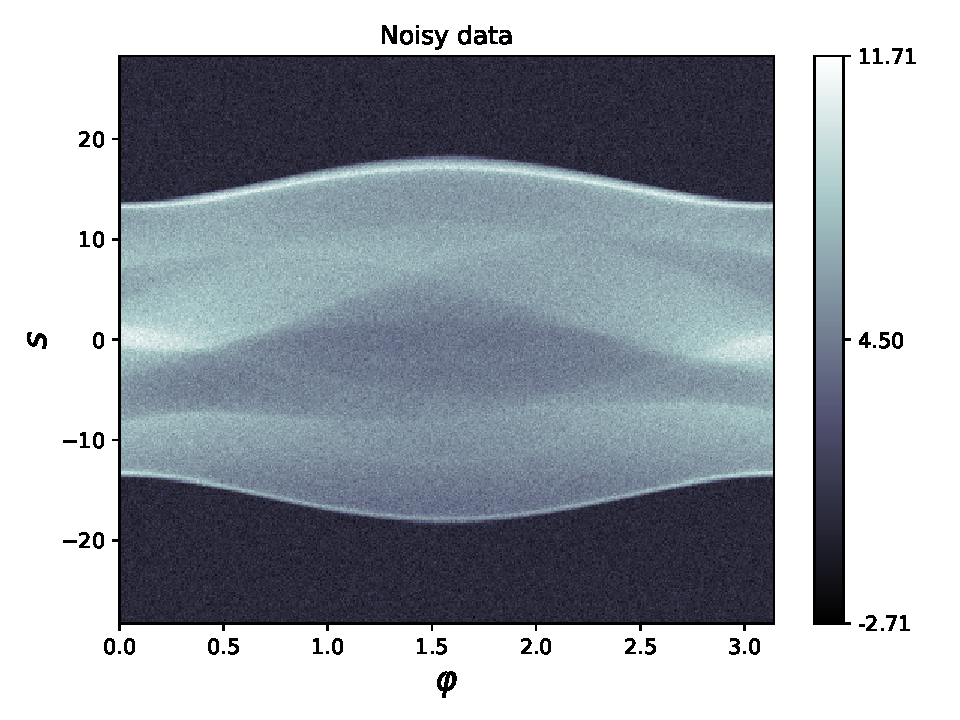
\includegraphics[width=\linewidth]{images/noisy_data_tv}
	\end{minipage}
	%
	\hspace*{0.01\linewidth}
	%
	\begin{minipage}{0.31\textwidth}
		\centering
		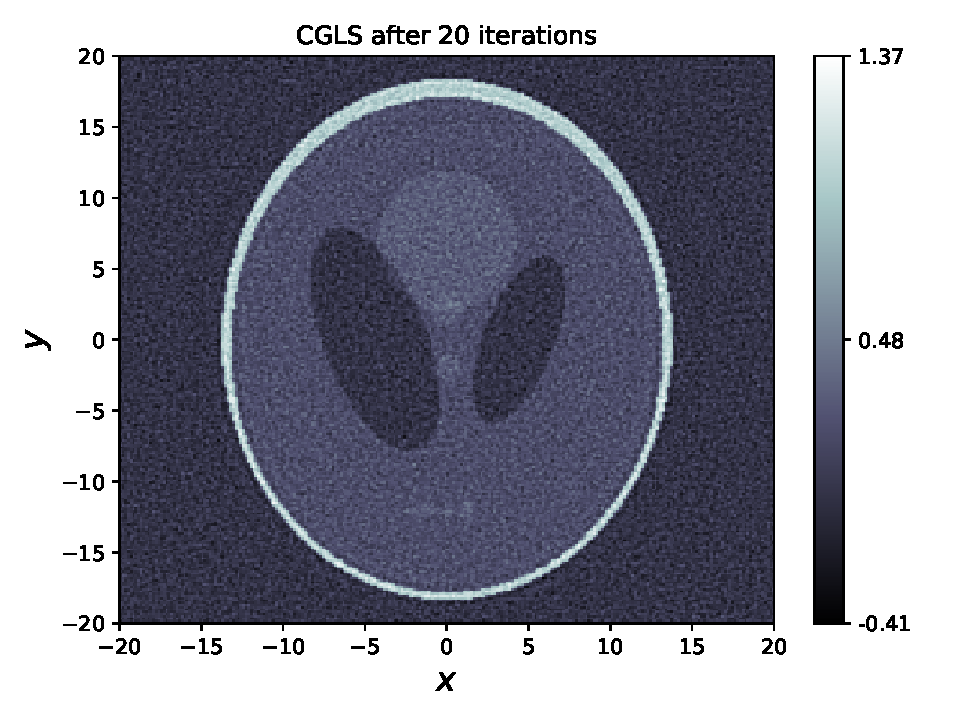
\includegraphics[width=\linewidth]{images/tomo_cgls_result.pdf}
	\end{minipage}
	
\end{frame}

\begin{frame}{Conclusions and Outlook}
	\begin{itemize}
		\item<+-> Reproducible -- scalable research requires rethinking scientific software
		\item<+-> ODL aims to solve these problems
		\item<+-> Well tested, used in $\approx$20 articles the last year
		\item<+-> Anyone is welcome to use and/or contribute!
	\end{itemize}
	\vspace{10mm}
	\begin{center}
		{\Huge \texttt{github.com/odlgroup/odl}}
	\end{center}
\end{frame}

\end{document}







